\documentclass[a4paper,12pt]{report}

% Language support
\usepackage[english,czech]{babel} % Primary language is English
\usepackage[T1]{fontenc}
\usepackage[utf8]{inputenc}

% Mathematical packages
\usepackage{amsmath, amssymb, mathrsfs, esdiff}

% Formatting and layout
\usepackage{geometry}
\geometry{verbose,tmargin=1.5cm,bmargin=2cm,lmargin=2cm,rmargin=2cm}
\usepackage{indentfirst}
\usepackage{calc}
\usepackage{enumitem}
\usepackage{array}
\usepackage{float}
\usepackage{fancyhdr}
\usepackage{mathrsfs} 
\pagestyle{plain}

% Hyperlinks
\usepackage{hyperref}
\hypersetup{
    colorlinks=true,
    citecolor=blue,
    filecolor=blue,
    linkcolor=blue,
    urlcolor=blue
}

% Graphics and tables
\usepackage{graphicx, epsfig, adjustbox, svg}
\usepackage[export]{adjustbox}
\usepackage{caption, subcaption}
\usepackage{booktabs}
\captionsetup[table]{skip=10pt}
\usepackage{multirow}
\usepackage{siunitx}

% Code highlighting
\usepackage{listings}
\usepackage{xcolor}
\lstset{
    language=Python,
    basicstyle=\ttfamily\small,
    keywordstyle=\color{blue},
    stringstyle=\color{red},
    commentstyle=\color{gray},
    numbers=left,
    numberstyle=\tiny\color{gray},
    stepnumber=1,
    numbersep=5pt,
    backgroundcolor=\color{lightgray!20},
    frame=single,
    breaklines=true,
    showspaces=false,
    showstringspaces=false,
    showtabs=false,
    tabsize=4,
    captionpos=b
}

% PDF inclusion
\usepackage{pdfpages}

% Customization of section titles
\addto\captionsenglish{
    \renewcommand{\listfigurename}{List of Figures}
    \renewcommand{\listtablename}{List of Tables}
    \renewcommand{\contentsname}{Contents}
    \renewcommand{\chaptername}{Chapter}
}

% Page and paragraph formatting
\setlength{\parindent}{15pt}
\setlength{\parskip}{4pt}
\frenchspacing

% Optional imports for advanced functionality
\usepackage{rotating} % Rotating objects
\usepackage{footmisc} % Advanced footnote options
\usepackage{gensymb}  % Degree symbol and similar

% Optional: header and footer customization (remove if not needed)
\lhead{}
\chead{}
\rhead{}
\lfoot{}
\cfoot{\thepage}
\rfoot{}
\renewcommand{\headrulewidth}{0pt}
\renewcommand{\footrulewidth}{0pt}




%----------------------------COMMANDY----------------------------------------------
\newcommand{\cvut}{České vysoké učení technické v Praze }
\newcommand{\fjfi}{Fakulta jaderná a fyzikálně inženýrská}
\newcommand{\kdaiz}{Katedra fyziky}
\newcommand{\studijniprogram}{Jaderná a částicová fyzika}
\newcommand{\nazeven}{Propagation of ultra-high energy cosmic rays in the Universe for the case of heavy composition of primary particles}    
\newcommand{\nazevcz}{}  
\newcommand{\autor}{Martin Šmíd}      
\newcommand{\rok}{2023/2024}        
\newcommand{\vedouci}{}     
\newcommand{\pracoviste}{FZÚ AV ČR} 
\newcommand{\klicova}{k}  
\newcommand{\keyword}{U}
\newcommand{\konzultant}{asi taky Ing. Alena Bakalová, Ph.D.} 
\newcommand{\abstrCZ}{K } 

\newcommand{\abstrEN}{Cosmic rays, discovered over a century ago, continue to be a phenomenon surrounded by unresolved questions. One of the primary questions is how these particles can be accelerated to ultra-high energy cosmic rays (UHECR), i.e. cosmic rays with $E \ge 10^{18}$~eV, and what processes contribute to their origin. To determine the sources of UHECRs, it is essential to study how cosmic rays evolve as they propagate through the universe.  It is believed that sources of UHECRs are of extragalactic origin. Therefore, they are influenced by various processes during their propagation in both galactic and extragalactic space.

This work focuses on the effects of cosmic ray propagation through the universe, particularly on the energy losses that occur due to interactions with ambient photon fields. Using Monte Carlo simulations, we identify the characteristics of cosmic ray sources capable of producing the heavy primary particles observed on Earth at the highest energies. }
\hypersetup{
 colorlinks=false,
 linkbordercolor={0 0 1},
 citebordercolor={0 0 1},
 urlbordercolor={0 0 1},
}

\newcommand{\na}[1]{\ensuremath{^{#1}}}


\begin{document}
	
\thispagestyle{empty}
%------------------------------------ÚVODNÍ STRANA------------------------------------
\begin{center}
  {\Large \bf \cvut\\[2mm] \fjfi\\ }
  \vspace{3mm}
  
  {\large \bf \kdaiz}\\
   \vspace{2mm} 
%  {\bf Obor: \obor}\\
  
  \vspace{0mm}

\begin{figure}[h]
\begin{center}
	
\includegraphics[scale=1.5]{cvut.jpg}
	% Je potřeba si stáhnout znak ČVUT a přidat ho k tomu souboru
\end{center}
\end{figure}

  \vspace{5mm}

%  {\LARGE \bf \nazevcz\vspace{8mm}\par \Large \nazeven}

  \vspace{0mm}
  {\Huge\textbf{Bakalářská práce}}

  \vspace{15mm}
  {\Large \textbf{\nazevcz}} \par 
  \vspace{15mm}
  {\Large \textbf{\nazeven}}
  
\end{center}

  \vfill
  {\large
  \begin{tabular}{ll}
  Autor: & \autor\\
  Vedoucí: & \vedouci\\
  Akademický rok: & \rok
  \end{tabular}
  }
% \end{center}
%-------------------------------------------------------------------------------------------------

\newpage 
\thispagestyle{empty} 


\noindent

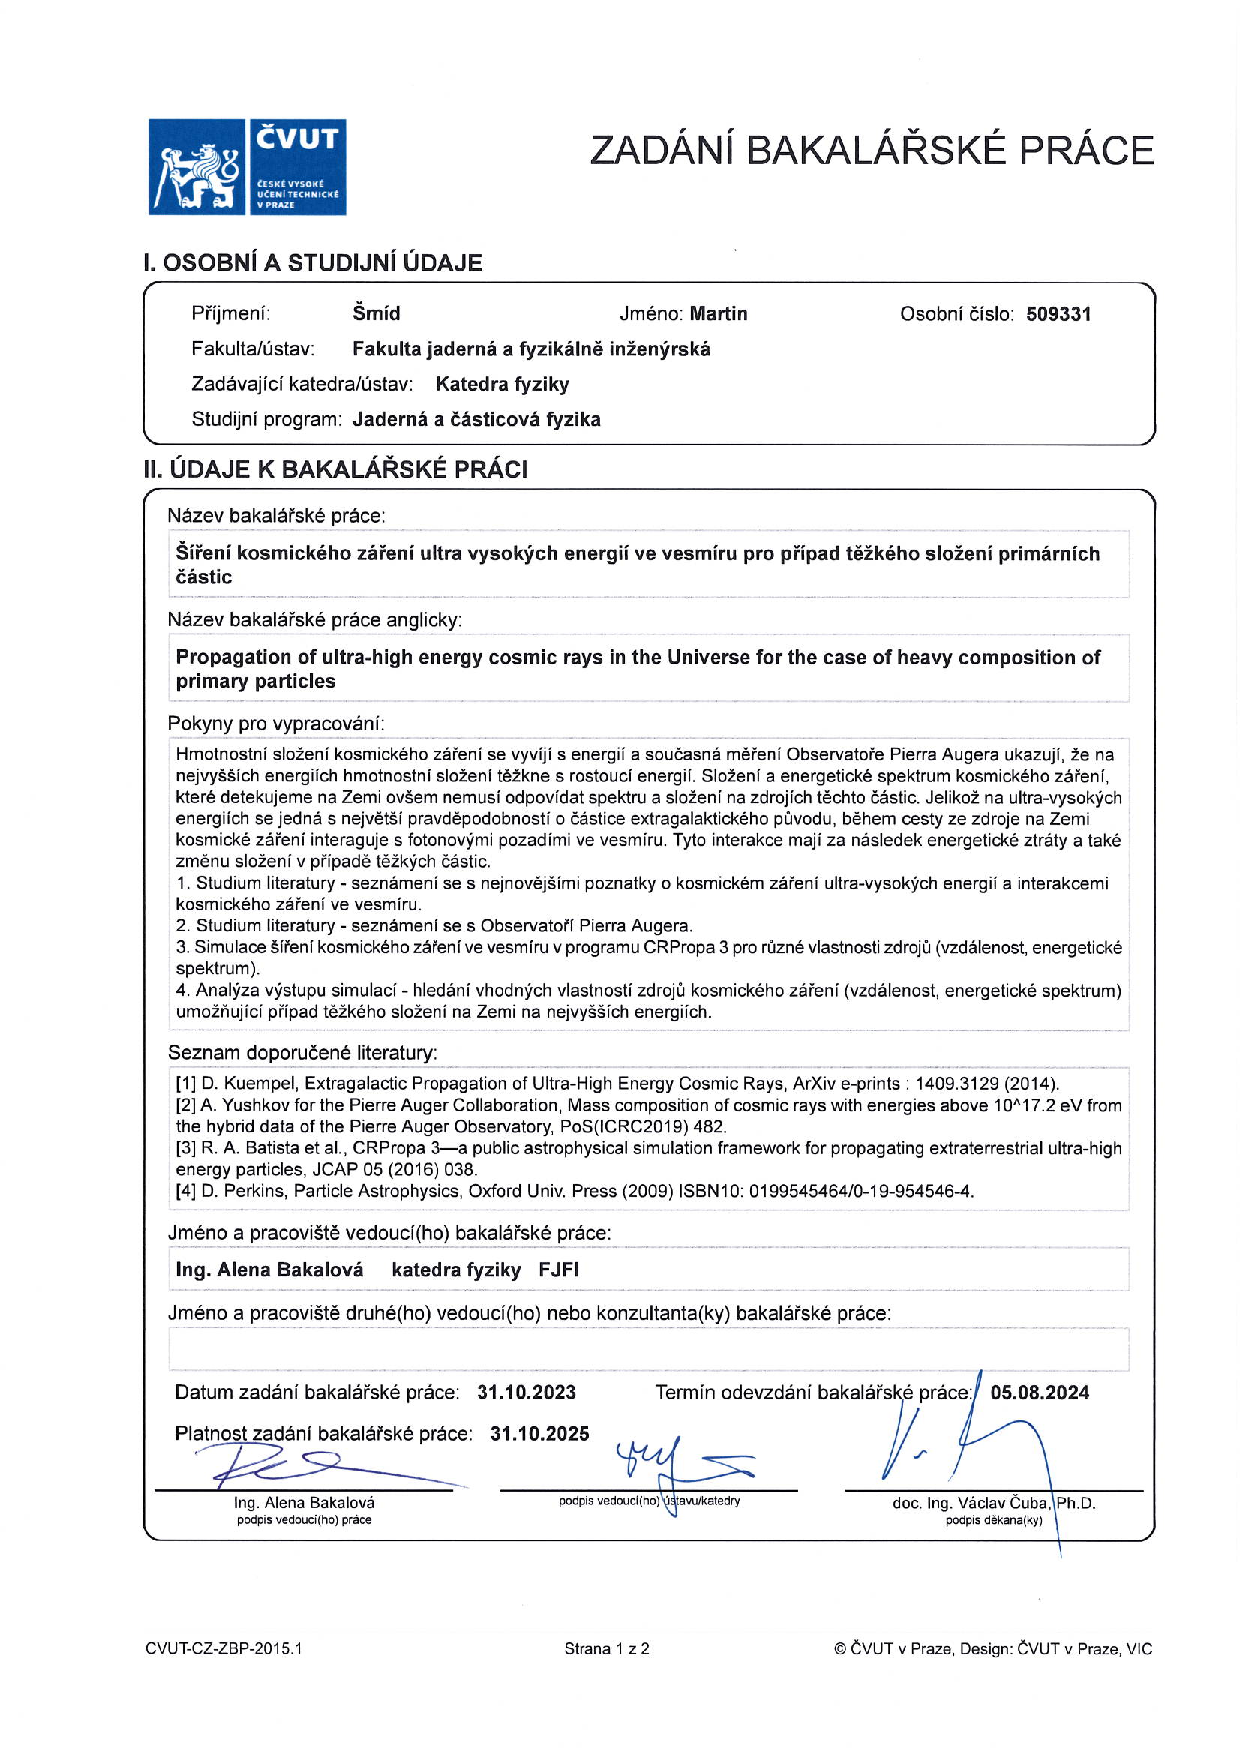
\includepdf[pages={-}]{zadání/smid.pdf}

\newpage 
\thispagestyle{empty} 
%---------------------------------------------------------------------------------------------

\newpage 
\thispagestyle{empty} 


\noindent

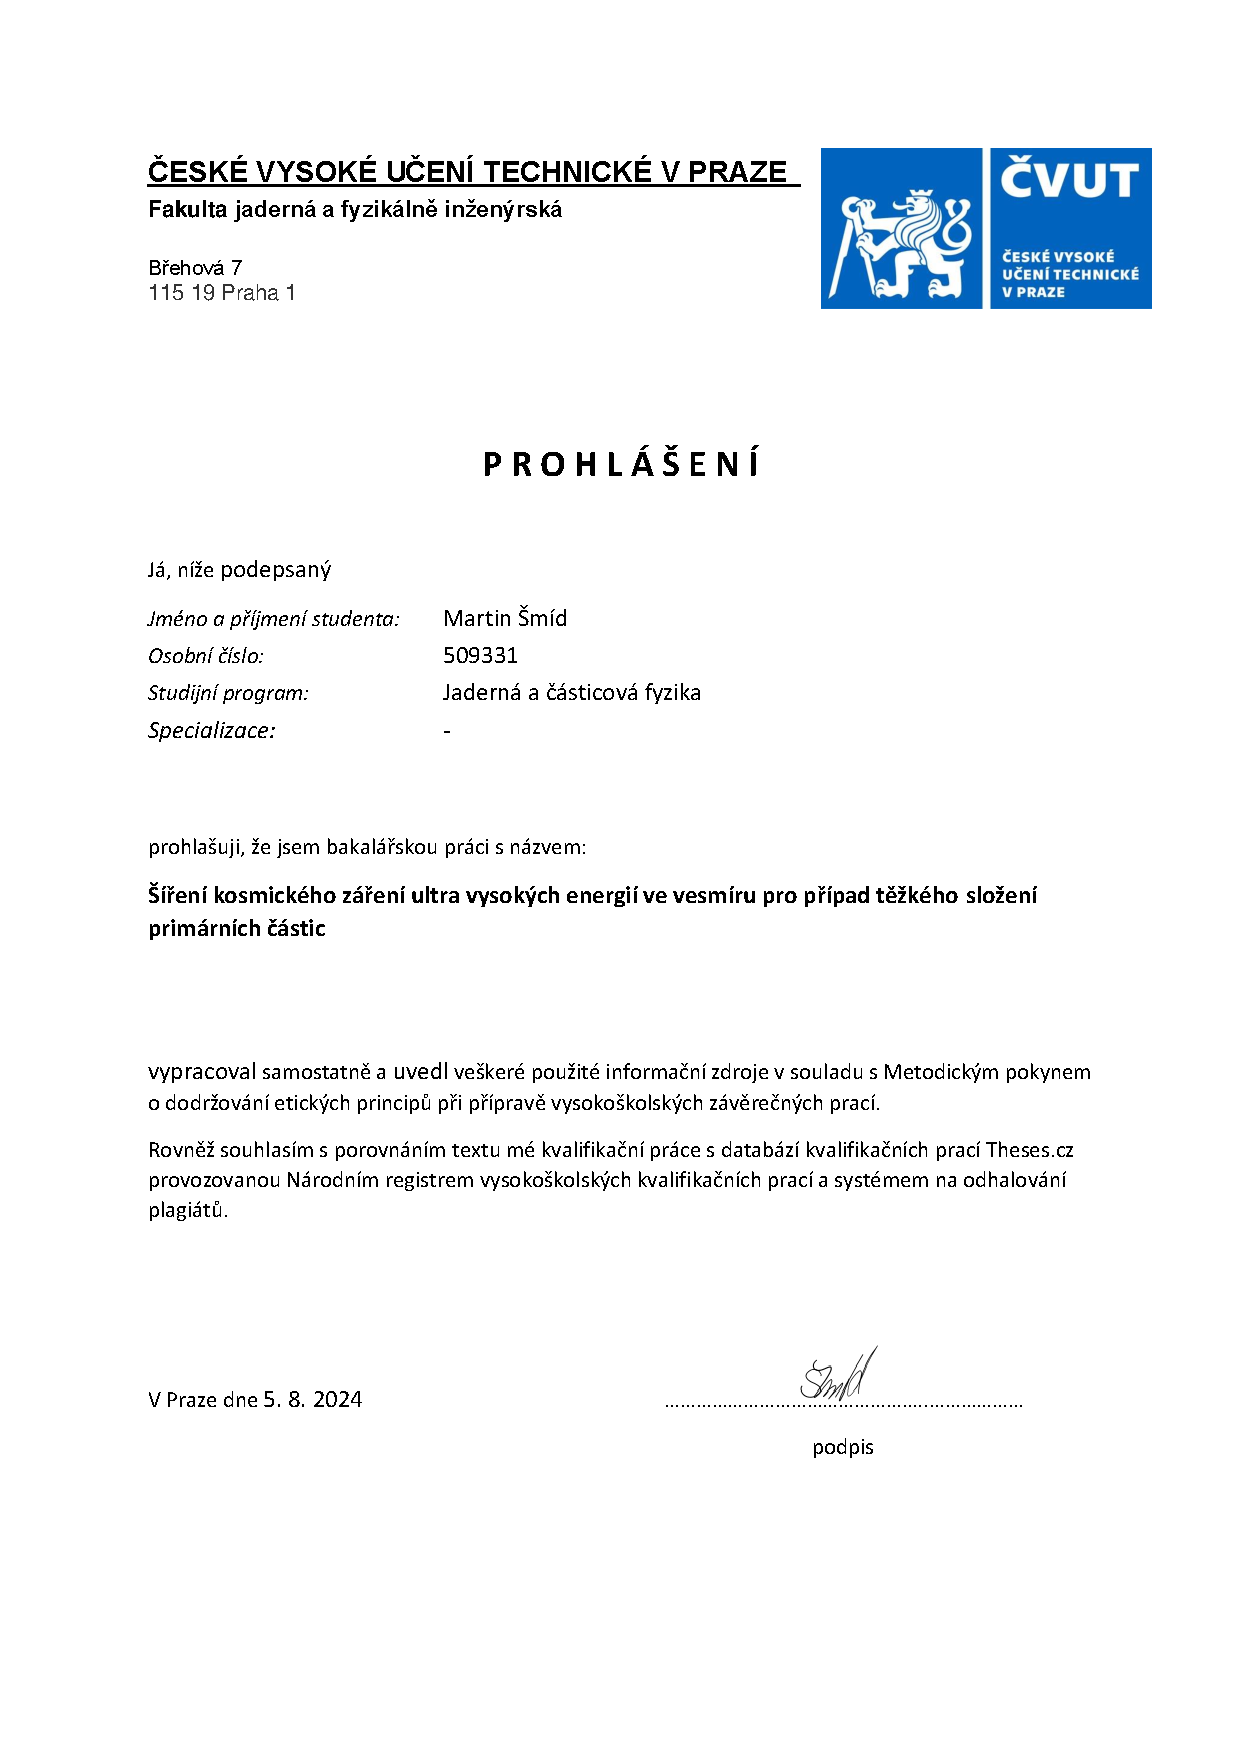
\includepdf[pages={-}]{zadání/BP_Prohlaseni_o_samostatnem_vypracovani_podepsano.pdf}

\newpage 
\thispagestyle{empty} 
%----------------------------------------------------------------

           
              

%---------------------------------------------------------------------------------------


\newpage
\thispagestyle{empty}

{
	\setlength{\parindent}{0pt}
	
	\textit{Název práce:}
	\textbf{\nazevcz} \\
	\textit{Autor:} \autor \\Moja bakalářka (Copy)
	\textit{Studijní program:} \studijniprogram \\
	
	\textit{Druh práce:} Bakalářská práce \\
	
	\textit{Vedoucí práce:} \vedouci, \pracoviste \\
	
	
	
	\textit{Abstrakt:} 
	\abstrCZ \\
	
	\textit{Klíčová slova:} \klicova
}
%----------------------------------------------------------------------------------
\newpage
\thispagestyle{empty}
{
	\setlength{\parindent}{0pt}
\textit{Title:}
\textbf{\nazeven} \\

\textit{Author:} \autor \\

\textit{Abstract:} 
\abstrEN \\

\textit{Key words:} \keyword
}

\newpage 
\thispagestyle{empty} 


~ 
\vfill 

{\bf \noindent Poděkování} 

\vspace{0.5cm} 
Rád bych poděkoval své vedoucí bakalářské práce, paní Ing. Aleně Bakalové, Ph.D., za její neocenitelnou pomoc, ochotu a především trpělivost, kterou mi věnovala při tvorbě této práce.


\tableofcontents
%-------------------------------------------------------------------------------------
\newpage


%------------------------------------------------------------------------------------
\newpage



\newpage  

%\chapter*{Úvod}
%  XXXXXXXXXXXXXXXXXXXXXXX
%
%\newpage

\chapter*{Introduction}
    \section*{Phase 0: Solving the Schrödinger vacuum equation}

Equation:
\begin{equation}
    i \frac{\partial \psi(x,t)}{\partial t} = - \frac{1}{2} \partial_x \psi(x,t)
\end{equation}
Dividing this by $\psi$ and integrating over time we get: 
\begin{equation}
    \int \frac{\partial \psi}{\psi} = \int A \partial t \xrightarrow{\text{which leads to:}} \psi(x,t+h) = \text{e}^{\int A} \psi (x,t) = e^{\int i \frac{1}{2} \partial^2_x \text{d}t}\psi(x,t)
\end{equation}
The exponential term can be expanded using Taylor series:
\begin{equation}
    e^{\int i \frac{1}{2} \partial^2_x \text{d}t} = 1 + \partial^2_x + \frac{\partial^4_x}{2} + \dots
\end{equation}
To which we can apply Furier transform, where derivation simply become multiplication by a parameter, and again using Taylor series we get:
\begin{equation}
    \widetilde{\psi}(x,t+h) = e^{\int i \frac{h}{2} k^2 \text{d}t}\widetilde{\psi}(x,t)
\end{equation}
Then we can simply use inverse Furier transform:
\begin{equation}
    \psi(x,t+h) = \mathscr{F}^{-1} \left[ e^{\int i \frac{h}{2} k^2 \text{d}t}\widetilde{\psi}(x,t) \right] 
\end{equation}

In code for simplicity, initial conditions are chosen to be: 
\begin{itemize}
    \item Boundaries: <a = 0, b = 1>
    \item Weave function: Complex Gausssian \begin{equation}
        \psi_0 (x) = A \cdot e^{-\frac{(x-x_0)^2}{2\sigma^2_0}} e^{ik_0 x}
    \end{equation}
    \item With $x_0 = 0.5$, $\sigma_0 = 0.1$ and initial momenta $k_0 = 0$
\end{itemize}

\section*{Phase 1: Solving the Schrödinger equation dependent on $r^2$}

We include the harmonic potential given by:
\begin{equation}
    V(r) = \frac{1}{2}  \omega^2 r^2 \hspace{0.5cm} \text{with} \hspace{0.5cm} r^2 = x^2 + y^2 + z^2.
\end{equation} 
For simplicity, we begin with a two-dimensional system ($n_x$ and $n_y$), and assume natural units where $\hbar = 1$, $m = 1$, and $\omega = 1$. The equation to solve is as follows:

\begin{equation}
-i \hbar \frac{\partial \Psi}{\partial t} = -\frac{\hbar^2}{2m} \nabla^2 \Psi + \frac{1}{2}m \omega^2 (x^2 + y^2 + z^2)\Psi,
\end{equation}


\subsection*{Analytical Solution}

The analytical solution for this system can be expressed in terms of Hermite polynomials and Gaussian functions. The stationary wave functions are as follows:

\begin{equation}
\psi_s(x, y, z) = C(n_x, n_y, n_z) H_{n_x}(x) H_{n_y}(y) H_{n_z}(z) 
\times e^{-\frac{\beta^2 (x^2 + y^2 + z^2)}{2}},
\end{equation}


where $H_{n}(x)$ are Hermite polynomials of order $n$, and $C_{n_x, n_y,n_z}$ is a normalization constant given by:

\begin{equation}
C(n_x, n_y, n_z) = \left(\frac{\beta^2}{\pi}\right)^{3/4} \frac{1}{\sqrt{2^{n_x + n_y + n_z} n_x! n_y! n_z!}},
\end{equation}
\begin{equation}
\beta = \sqrt{\frac{m \omega}{\hbar}}.
\end{equation}




\subsection*{Numerical Approach}

We solve the Schrödinger equation using a split-step Fourier method. The approach involves alternating between applying the kinetic energy operator in Fourier space and the potential energy operator in real space. The evolution of the wave function over a small time step $h$ is given by:

\begin{equation}
\psi(x,y,t+h) = e^{-i \frac{h}{2} \nabla^2} e^{-i h V(x,y)} e^{-i \frac{h}{2} \nabla^2} \psi(x,y,t).
\end{equation}

\subsubsection*{Initial Conditions}

For now the work is done on a 2D Gaussian wave packet:

\begin{equation}
\psi_0(x, y) = A \cdot e^{-\frac{(x-x_0)^2 + (y-y_0)^2}{2\sigma^2}} e^{i(k_x x + k_y y)},
\end{equation}

with $x_0 = 0.5$, $y_0 = 0.5$, $\sigma = 0.1$, and initial momenta $k_x = 0$, $k_y = 0$. The boundaries of the domain are set to $x, y \in [0, 1]$.

\subsubsection*{Error Analysis}

To assess the accuracy of the numerical solution, two types of errors must be monitored:

Error in the Wavefunction:
\begin{equation}
\text{Err}{\psi} = \left| \psi_{\text{numerical}}(x,y,t) - \psi_{\text{analytical}}(x,y) \right|.
\end{equation}
This measures the deviation of the numerical solution from the analytical stationary solution.

Error in the Probability Density:
\begin{equation}
\text{Err}{\rho} = \left| \left| \psi_{\text{numerical}}(x,y,t) \right|^2 - \left| \psi_{\text{numerical}}(x,y,t=0) \right|^2 \right|.
\end{equation}
As the analytical solution is stationary, the probability density $|\psi|^2$ should remain constant over time. Any deviation provides a measure of the numerical error.






%--------------------------------------------SEM NESAHAT-----------------------------









\bibliographystyle{JHEP}
\bibliography{bibliography}

\end{document} 
